
\section{Architecture Integration}

\subsection{Model Support}

\begin{table}[H]
\centering
\small
\begin{tabular}{llllll}
\toprule
\textbf{Model} & \textbf{Attention class} & \textbf{Nested?} & \textbf{RoPE?} & \textbf{GQA?} & \textbf{Verified} \\
\midrule
DistilBERT & \texttt{MultiHeadSelfAttention} & No & No & No &  \\
RoBERTa & \texttt{BertSelfAttention} (nested) & Yes & No & No &  \\
GPT-2 & \texttt{GPT2Attention} (Conv1D) & No & No & No &  \\
Qwen3.5 & \texttt{Qwen3Attention} & No & Yes & Yes & 0.85 \\
\bottomrule
\end{tabular}
\end{table}

\subsection{Weight Extraction}

\subsubsection{DistilBERT}

\begin{lstlisting}
extracted["q"] = src.q\_lin.weight
extracted["k"] = src.k\_lin.weight
extracted["v"] = src.v\_lin.weight
extracted["o"] = src.out\_lin.weight
\end{lstlisting}

\subsubsection{RoBERTa (nested)}

\begin{lstlisting}
s = src.self
extracted["q"] = s.query.weight
extracted["k"] = s.key.weight
extracted["v"] = s.value.weight
extracted["o"] = src.output.dense.weight
\end{lstlisting}

\subsubsection{GPT-2 (Conv1D)}

\begin{lstlisting}
w = src.c\_attn.weight.t()
q\_w, k\_w, v\_w = w.chunk(3, dim=0)
extracted["q"] = q\_w
extracted["k"] = k\_w
extracted["v"] = v\_w
extracted["o"] = src.c\_proj.weight.t()
\end{lstlisting}

\subsubsection{Qwen}

Direct extraction from \texttt{q\_proj/k\_proj/v\_proj/o\_proj}.

\subsection{Hybrid Initialization}

SVD-Mamba's \texttt{copy\_weights} does three things:

\begin{enumerate}
\item \textbf{Attention path:} Factorize $W_Q, W_K, W_V, W_O$ into SVD factors
  for the attention projections.
\item \textbf{SSM input projection:} Build a concatenated $[V; Q]$ weight to
  initialize \texttt{in\_proj}.
\item \textbf{Output projection:} Copy the attention out projection to \texttt{attn\_out\_proj}.

\end{enumerate}
\textbf{The SSM branch is NOT initialized from the attention weights.} It starts 
with random weights, but its contribution is silenced by the gate.

\subsection{The Gating Module}

\begin{lstlisting}
self.gating = nn.Linear(self.d\_model, self.d\_model)
nn.init.zeros\_(self.gating.weight)
nn.init.constant\_(self.gating.bias, -7.0)
\end{lstlisting}

\textbf{Why bias $-7$?} The gating controls the SSM path:

\begin{itemize}
\item $\sigma(-7) \approx 0.0009$ $\to$ SSM contributes \textless{}0.1\% at start.
\item The model starts as pure attention.
\item During recovery, the gate can shift toward SSM.

\end{itemize}
\subsection{Nested Encoder Handling}

For RoBERTa/BERT, \texttt{is\_nested\_encoder = True} means SVD-Mamba returns the 
raw output. The outer \texttt{attention.output.dense} applies the actual output 
projection.

But note: SVD-Mamba's forward sets \texttt{is\_nested\_encoder = True} in the 
constructor if the source has the right structure, and the forward 
returns \texttt{Y} directly. There's no explicit bypass code -- the output 
shape is already \texttt{[B, L, d]}.

\subsection{Injection}

The injection hook handles:

\begin{itemize}
\item Whole-model traversal
\item Single layer replacement
\item Double-injection guard
\item Qwen DeltaNet skip

\end{itemize}
\begin{lstlisting}
def inject\_svd\_mamba(layer=None, model=None, ...):
    target = layer or model
    
    # Whole model
    if isinstance(target, nn.Module) and has\_transformer\_layers(target):
        for lyr in layers:
            inject\_svd\_mamba(layer=lyr, ...)
        return target
    
    # Single layer
    src = find\_attention(target)
    new\_module = SVDMamba(d\_model=..., pretrained\_attn=src)
    replace\_attention(target, new\_module)
    return new\_module
\end{lstlisting}

\subsection{The Chunked SSM Scan}

The forward uses a Python loop over chunks:

\begin{lstlisting}
chunk\_size = 64
num\_chunks = (seqlen + chunk\_size - 1) // chunk\_size
h\_running = zeros(...)
h\_den\_running = zeros(...)
y\_chunks = []

for c in range(num\_chunks):
    s\_idx = c * chunk\_size
    e\_idx = min(seqlen, s\_idx + chunk\_size)
    
    u\_c = u[:, s\_idx:e\_idx]
    log\_a\_c = log\_alpha[:, s\_idx:e\_idx]
    lambda\_c = cumsum(log\_a\_c, dim=1).clamp(min=-25, max=0)
    
    decay\_c = exp(lambda\_c)
    decay\_inv\_c = exp(-lambda\_c).clamp(max=1e10)
    
    h\_intra = decay\_c * cumsum(decay\_inv\_c * u\_c, dim=1)
    h\_inter = decay\_c * h\_running.unsqueeze(1)
    h\_chunk = (h\_intra + h\_inter).clamp(min=-1e4, max=1e4)
    
    # ... denominator ...
    y\_chunks.append(...)
    h\_running = h\_chunk[:, -1]
\end{lstlisting}

\textbf{Python loop overhead} is significant: for $L = 128$, 2 iterations; for 
$L = 1024$, 16 iterations. Each iteration has $\sim 10$ kernel launches.

\subsection{Numerical Stability}

Several clamps prevent overflow:

\begin{table}[H]
\centering
\small
\begin{tabular}{ll}
\toprule
\textbf{Operation} & \textbf{Clamp} \\
\midrule
\texttt{log\_alpha} cumsum & $[-25, 0]$ \\
\texttt{h\_chunk} & $[-10^4, 10^4]$ \\
\texttt{h\_den\_chunk} & $[0, 10^4]$ \\
\texttt{decay\_inv} & $\leq 10^{10}$ \\
\texttt{denom} & $\geq 10^{-4}$ \\
\texttt{A\_log} & $[-20, 10]$ \\
\bottomrule
\end{tabular}
\end{table}

\subsection{Registry}

\begin{lstlisting}
@ATTENTION\_REGISTRY.register("svd\_mamba")
@ATTENTION\_REGISTRY.register("SVD-Mamba")
@ATTENTION\_REGISTRY.register("svd-mamba")
@ATTENTION\_REGISTRY.register("SVD\_Mamba")
class SVDMamba(BaseAttention):
    ...
\end{lstlisting}

\subsection{Failure Modes}

\begin{table}[H]
\centering
\small
\begin{tabular}{lll}
\toprule
\textbf{Failure} & \textbf{Detection} & \textbf{Response} \\
\midrule
Missing projection & \texttt{copy\_weights} raises & Injection aborts \\
Small Frobenius norm & Explicit check & Raises RuntimeError \\
NaN in scan & \texttt{torch.nan\_to\_num} & Fallback \\
OOM & RuntimeError & Reduce batch \\
Cross-attention & Returns input & No-op \\
\bottomrule
\end{tabular}
\end{table}

\subsection{Cross-Attention}

If \texttt{encoder\_hidden\_states} is provided, SVD-Mamba returns 
\texttt{(hidden\_states, None)} -- a pass-through. This means cross-attention is 
effectively unsupported.
\begin{lstlisting}

---
\end{lstlisting}

\begin{figure}[H]
\centering
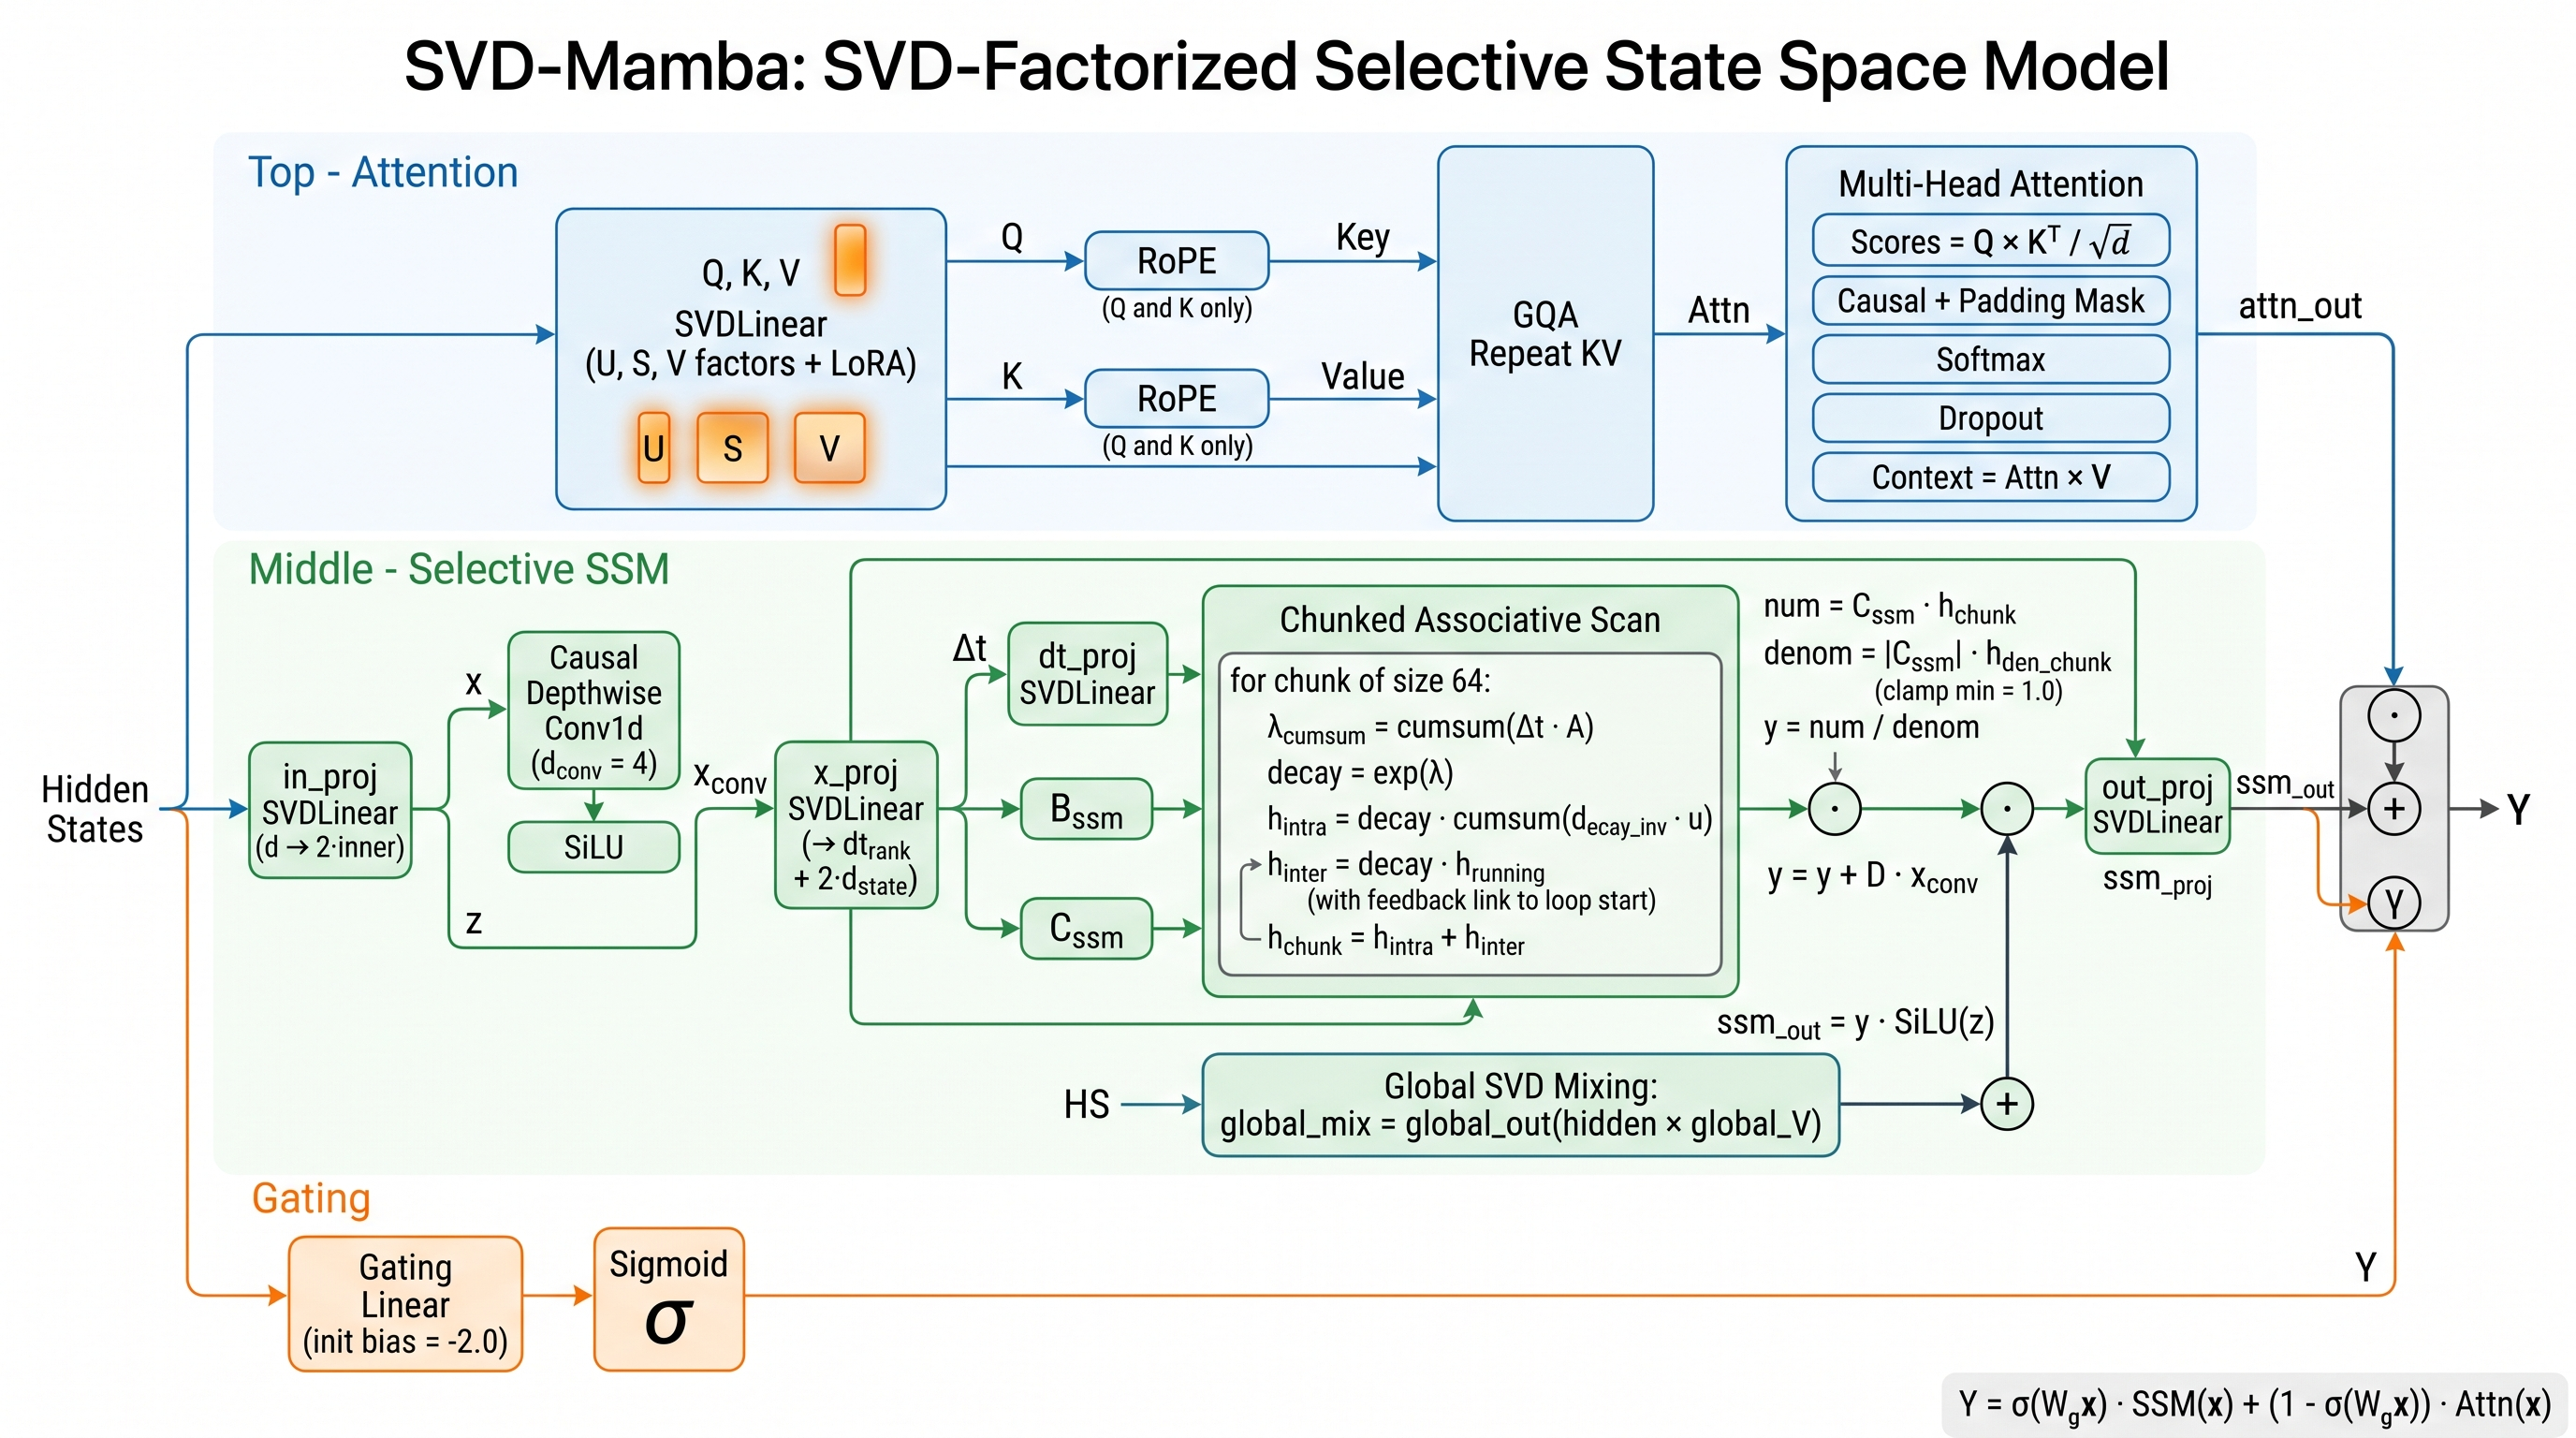
\includegraphics[width=\linewidth]{figures/architecture.jpeg}
\caption{High-level architectural diagram of svd\_mamba.}
\label{fig:arch\_svd-mamba}
\end{figure}

